
The experiment from which the parameters are derived employs bioengineered micropatterning techniques
to create a regular arrangement of circular ‘patches’ that are populated with cells surrounded by bare substrate. The non-populated regions emulate necrotic regions of the retina that result from repeated exposure to reactive oxidative species, triggering neovascularization and exudative AMD \cite{Chopdar2003Age}.  Recreating these regular spatially organized cellular configurations is essential to understanding the impact that local cell-cell and cell-environment interactions has on VEGF autoregulation. In the experimental study, described in \cite{qanitabaker:Vargis2014Effect}, the bioengineered circular micro patterns are employed to control the extent of cell-cell interactions, which occur within the patch, and cell-environment interactions, which occur at the perimeter. Several patch sizes were used in this study \SI{100}{\micro\metre}, \SI{200}{\micro\metre}, \SI{300}{\micro\metre}, and \SI{400}{\micro\metre} to vary the mix of cell-cell and cell-environment in each experiment and constrain the possible parameter values. Each patch was seeded with retinal pigment epithelial (RPE) cells and grown in a cellular culture. As the cells grow the VEGF per cell was measured at regular intervals: 4, 24, 30 48, 54, 72 hours. To measure the VEGF per cell, enzyme-linked immunosorbent assay (ELISA) determined the total VEGF contained within the cell culture and the number of cells per patch was determined by image analysis proceeded by staining. Figure~\ref{in_vitro_experiment}(a) (taken from \cite{qanitabaker:Vargis2014Effect}) illustrates the stained patches at 72 hours.

Experiments were repeated ten times and averaged. The final spatial-temporal data produced is illustrated in Figure~\ref{in_vitro_experiment}(b) and forms the target prediction for the computational model simulation that identifies the unknown parameters by minimizing matching simulated data spatial-temporal VEGF/cell levels.

The bioengineered experiments were simulated using a hybrid agent-based approach, which is an extension of \textsl{iDynoMiCs} framework developed by the Kreft group at University of Birmingham \cite{qanitabaker:Lardon2011IDynoMiCS}. Hybrid models integrate discrete components to represent the cells and continuous equations to represent biochemical reactions and diffusion. Each cell is represented as a spherical particle which grows by consuming nutrient and accumulating biomass volume; when the volume exceeds twice the initial volume cell division is simulated by splitting the particle into two. Particles can secrete and uptake soluble biochemicals (such as VEGF) which diffuses through the domain; regulatory reactions which model interactions among intracellular proteins are modeled as ODEs. Simulation interlaces cellular growth and movement (implemented by relaxing forces between particles) with biochemical redistribution (implemented by solving the PDEs). Random noise is added to cellular movement and split volume to represent inherent stochasticity of the biological processes.

The setup of the simulations replicates the same experimental conditions and units as in the \textit{in vitro} experiments. The domain size of each simulation is \SI{2400}{\micro\metre}, initial cell size is set to $80 \mu m^2$ and the doubling time due to growth is set at 36 hours. Each simulation begins with multiple RPE cells distributed at the reported patterning efficiency in several patches arranged in the specific experimental pattern. The simulation replicates the first 72 hours of the \textit{in vitro} experiments. Illustrations of the simulated experiments are shown in Figure~\ref{simulation_examples}.

This framework is inherently multiscale in that the parameters that control the low-level mechanisms at the cellular level, e.g., the VEGF secretion rate and autoregulation, determine the VEGF concentration over the complete domain, a multi-cellular property. Also, the VEGF concentration measured through several simulation time-slots represents the higher scale where treatment outcomes could be assessed. The VEGF gradients illustrated in \ref{simulation_examples} determine the final outcome of VEGF concentration per cell \cite{qanitabaker:Cao2007Spatiotemporal} and intrinsically include the quantitative spatiotemporal controls effects as the cells grow. In addition, the spatial gradients are implicitly considered due to the diffusive nature of the VEGF transport over the several experimental conditions (in this model, the different patch size experiments).

 \begin{figure}[!t]
  \centering

 \begin{subfigure}{.5\textwidth}
   \centering
   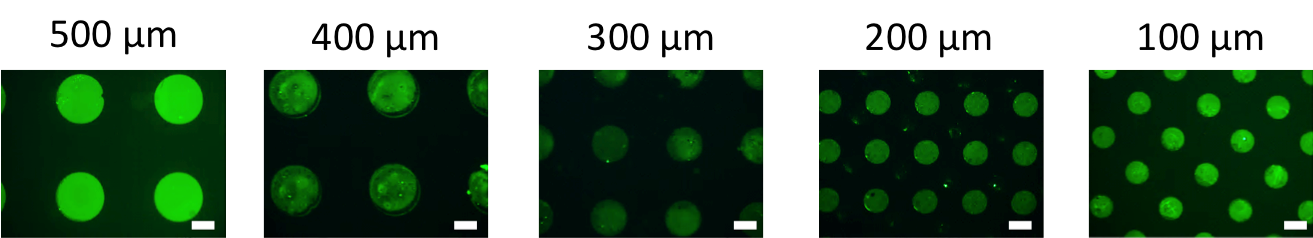
\includegraphics[width=.8\linewidth]{./figures/in_vitro_crop.png}
   \caption{(a) Patches of stained RPE cells at 72 hours for each patch size. \cite{qanitabaker:Vargis2014Effect}.}

 \end{subfigure}%

 \begin{subfigure}{.5\textwidth}
   \centering
   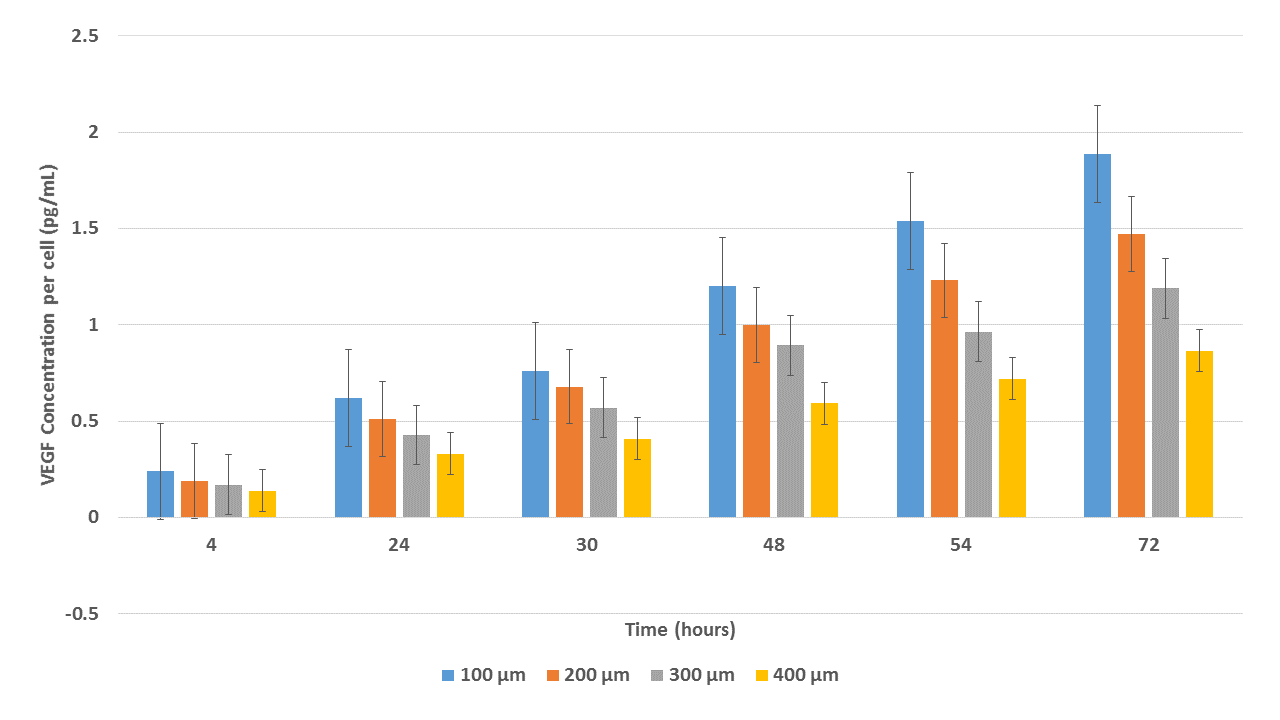
\includegraphics[width=.8\linewidth]{./figures/Results/In-Vitro.png}
   \caption{(b) Time course of VEGF expression per cell measured at 4, 24, 30, 48, and 72 h ( data for each time from the \textit{in vitro} \cite{qanitabaker:Vargis2014Effect} ).}
 \end{subfigure}%
\label{in_vitro_experiment}
\end{figure}

 The autoregulation of VEGF secretion as a function of biomass $M$ and local VEGF concentration $V$ is described using Equation ~\ref{VEGF_autoregulation}. The diffusion coefficient of VEGF $D_{V}$ is set to $5.8 \times 10^{-11} m^{2} s^{-1}$ taken from microfluidic experiments described in \cite{qanitabaker:Shin2012Microfluidic}.

 \begin{equation}
 \frac{\partial V}{\partial t}=D_{V}\bigtriangledown^{2} V+ \alpha_V  \frac{K_i}{ \beta V+K_i} M
 \label{VEGF_autoregulation}
 \end{equation}

Over time, the RPE cells grow based on doubling time 36 h \cite{qanitabaker:Bryckaert2000Regulation} with determines the growth rate parameter $\mu _{M}$. We applied first order kinetic for cells growth on the system as shown in Equation \ref{Cell_Growth}.\\


\begin{equation}
\frac{\partial M}{\partial t}=   \mu _{M} M
\label{Cell_Growth}
\end{equation}

Table \ref{parameters} summarizes the description of the parameters used in the equations above and identify those parameters whose value is known and those that need to be determined by the method introduced in this paper.

\begin{table}[ht]
\caption{ List of parameters symbol description } % title of Table
\centering
\begin{footnotesize}
\begin{tabular}{l l l}
\hline
Parameter   &  Value & Description\\ \hline \hline
$D_{V}$     & $5.8 \times 10^{-11} m^{2} s^{-1}$ & VEGF soluble factor diffusion coefficient\\
$\alpha_V $ & \textsl{Unknown}                   & Rate at which VEGF is secreted by the RPE \\
$\beta $    &  \textsl{Unknown}                  & The VEGF binding coefficient (VEGF binding affinity) \\
$K_i$       &  \textsl{Unknown}                  & The auto regulation rate of VEGF \\
$\mu _{M}$  &  ??????????????                    & Maximum specific rate for RPE cell growth \\
 [1ex]      % [1ex] adds vertical space
\hline 
\end{tabular}
\end{footnotesize}
\label{parameters} 
\end{table}

\begin{figure*}
 \begin{center}
  \begin{tabular}{cc}
   
\includegraphics[width=0.20\textwidth]{./figures/PatchCloseUp.png} &   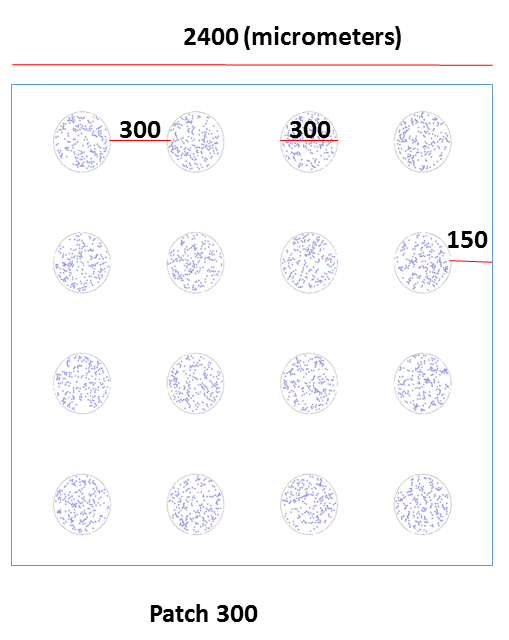
\includegraphics[width=0.20\textwidth]{./figures/Patch300.png} \\
   (a) & (b) \\
   
\includegraphics[width=0.20\textwidth]{./figures/VEGFCloseUp.png} &  
\includegraphics[width=0.20\textwidth]{./figures/VEGF300.png} \\
   (c) & (d)
   \end{tabular}
   \end{center}

\caption{(a) Closeup of initial condition of a $300 \mu \metre$ patch (b) Experiment with $300 \mu \metre$, 4 patches in each side. (c) Closeup of the VEGF distribution after 72 hours, (d) VEGF distribution over whole domain after 72 hours.  }
  \vspace{+1mm}
\label{simulation_examples}
\end{figure}



